\documentclass[oneside,11pt]{amsart}
\usepackage[utf8]{inputenc}%
\usepackage[english]{babel}%
\usepackage{amsmath,amssymb,amsthm,amsfonts}%
\usepackage[unicode]{hyperref}%
\usepackage{mathrsfs,bbm}%
\usepackage{paralist}
\usepackage{color}
\usepackage{longtable}
\usepackage{array}
\newcolumntype{L}[1]{>{\small\raggedright\arraybackslash}m{#1}}
\newcolumntype{T}[1]{>{\footnotesize\raggedright\arraybackslash}m{#1}}
\usepackage{stmaryrd}%
%\usepackage{refcheck}
\usepackage{graphicx}
\usepackage[DIV14]{typearea}
\usepackage{multicol,tikz}
\usepackage{datetime}
\usepackage{cleveref}

\usepackage[shadow]{todonotes}

\usepackage{etoolbox}
\patchcmd{\section}{\scshape}{\Large\itshape\bfseries}{}{}

\usepackage{caption}
\captionsetup{labelformat=empty,labelsep=none}

\hypersetup{
  colorlinks=true,
  linkcolor=blue!50!red,
  urlcolor=green!60!black
}

%%%%%%%%%%%%%%%%%%%%%%%%%%%%%%%%%%%%%%%%%%%%%%%%%%%%%%%%%%%%%%%%%%%%%%%%%%%%%%%%%%%%%%%%
\synctex=1
%%%%%%%%%%%%%%%%%%%%%%%%%%%%%%%%%%%%%%%%%%%%%%%%%%%%%%%%%%%%%%%%%%%%%%%%%%%%%%%%%%%%%%%%
%%%%%%%%%%%%%%%%%%%%%%%%%%%%%%%%%%%%%%%%%%%%%%%%%%%%%%%%%%%%%%%%%%%%%%%%%%%%%%%%%%%%%%%%
\newcommand{\score}[1]{\textit{#1}\addtocounter{totalscore}{#1}}
\newcommand{\razdel}[1]{\smallskip\underline{\textbf{#1:}}\smallskip}

\newcommand{\note}[1]{{\sf{}\color{blue}(#1)}}

\begin{document}

\title[MATH 7310: REAL ANALYSIS AND LINEAR SPACES I]{MATH 7310: REAL ANALYSIS AND LINEAR SPACES I}
\author{Leonid Petrov\\Spring 2020}
\date{Compiled on \today, \currenttime{} (in whatever timezone I was at that time).\\An up to date syllabus is always on \texttt{GitHub} at \url{https://github.com/lenis2000/Syllabi/blob/master/Syllabus_7310_s20.pdf}. For direct PDF download use \href{https://github.com/lenis2000/Syllabi/raw/master/Syllabus_7310_s20.pdf}{\texttt{this link}}.
	\LaTeX{} source with \textit{changes} to the syllabus is \href{https://github.com/lenis2000/Syllabi/blob/master/Syllabus_7310_s20.tex}{\texttt{here}}
(click ``History'').
\\Note that this PDF has green clickable links.}
\maketitle

\bigskip

\section{Graduate real analysis}
\bigskip

This course introduces students to fundamental analytic tools used across all of mathematics:
\begin{itemize}
	\item Measures, including the Lebesgue measure on the line
	\item Lebesgue integration
	\item $L^p$ and Hilbert spaces
	\item Absolute continuity, differentiation of measures
\end{itemize}

Additional topics included in the course will range from applications to
probability (e.g., theory of conditional expectations, Gaussian measures and Gaussian Free Field, \ldots)
to selected topics from classical analysis (orthogonal polynomials, numerical methods, steepest descent, \ldots),
as time permits.
Students' suggestions of additional topics are very welcome.

A central technical skill which you will develop is mathematical writing
and presentation of ideas. This goal is reflected in write-up tasks and
in grading of homeworks and midterms.

\begin{figure}[h]
	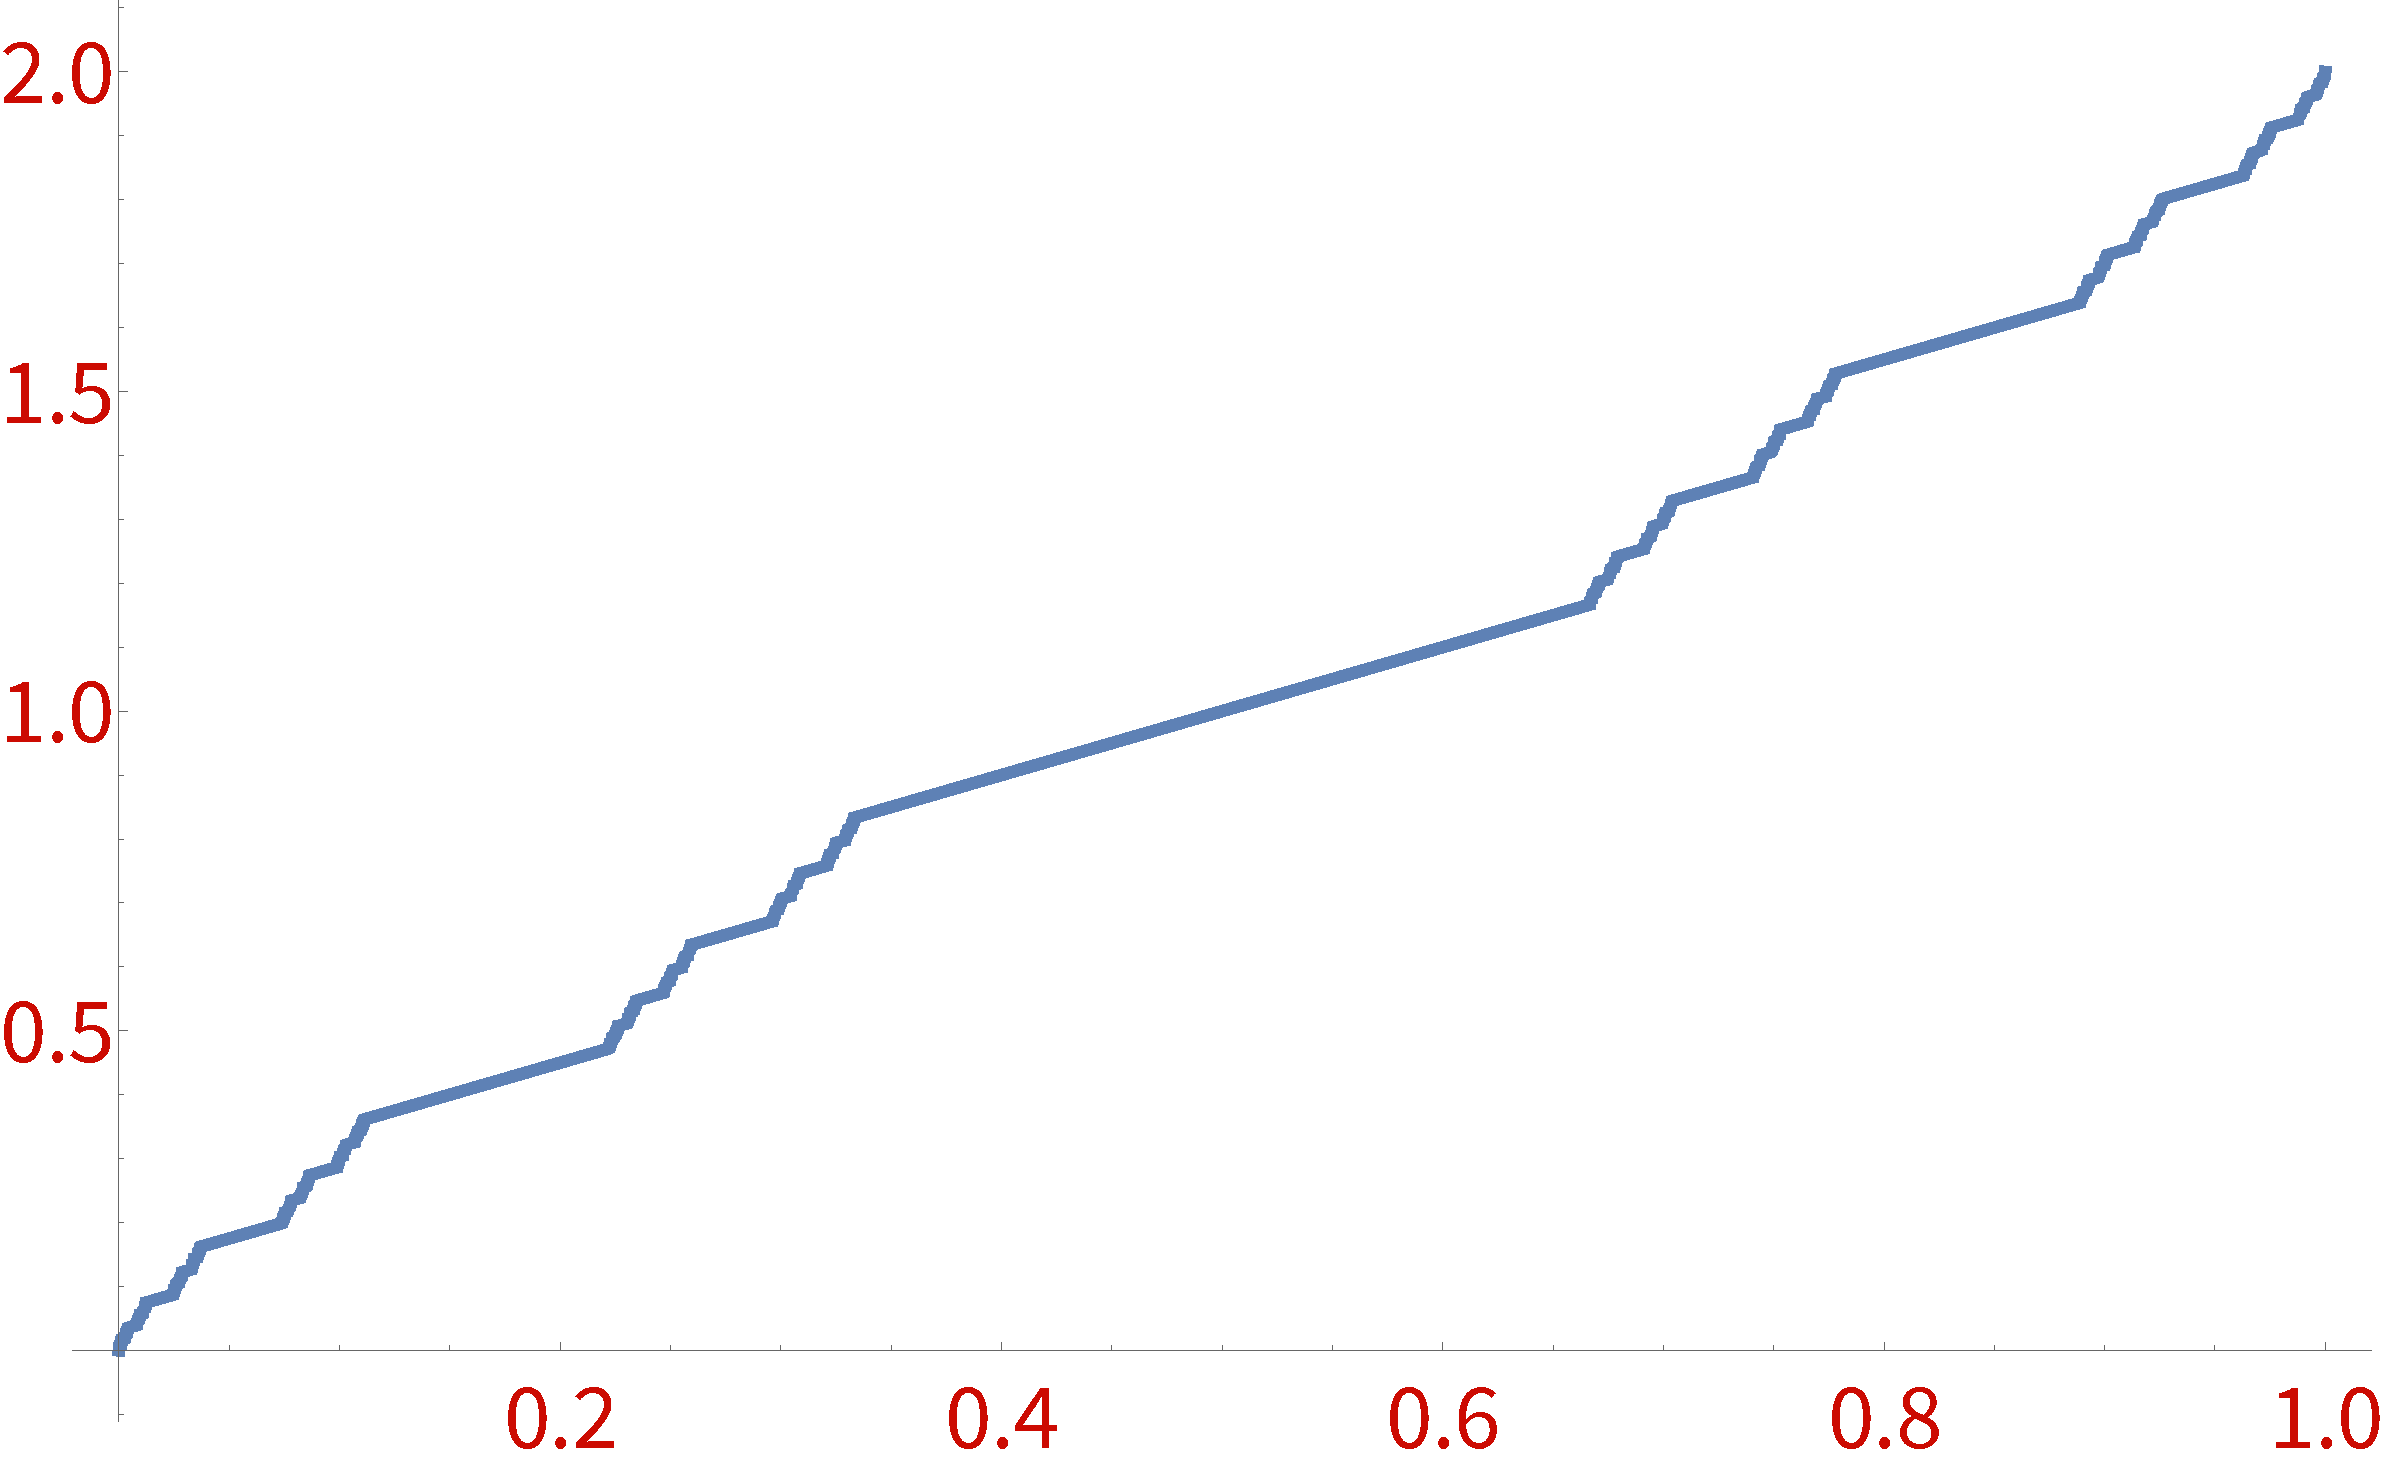
\includegraphics[height=.35\textwidth]{img/Cantor.pdf}
	\qquad 
	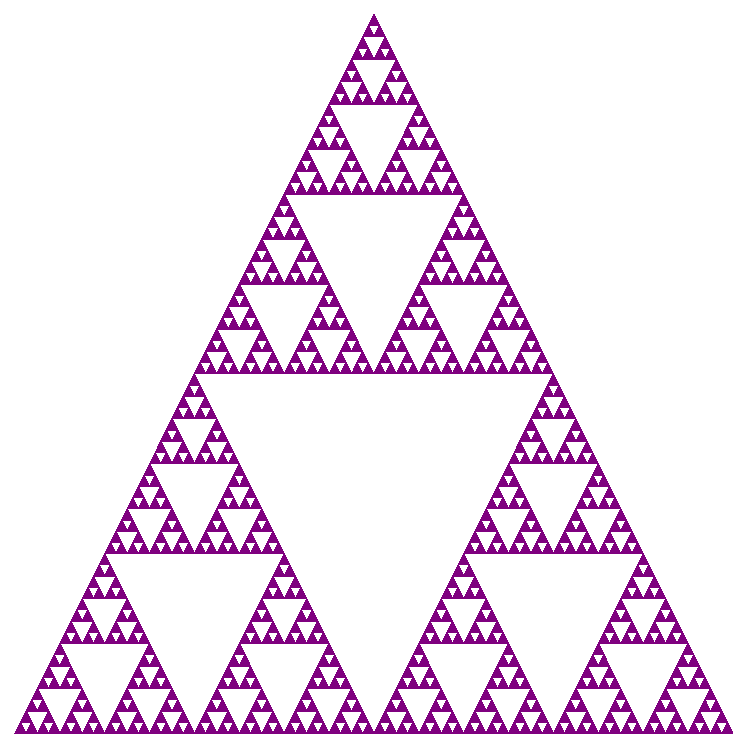
\includegraphics[height=.35\textwidth]{img/Sierp.pdf}
	\caption{Left: The cantor ladder plus $x$, an important counterexample in the course.\\
	Right: The Sierpinski triangle, a fractal set whose area you will be able to compute.}
\end{figure}

\subsection*{Prerequisites}

Single variable and multi-variable Calculus (limits and continuity,
differentiation and integration, series, uniform convergence, etc.), Linear
Algebra (vector spaces, linear mappings, matrices, determinants, etc.), and
some knowledge of set theory and topology of metric spaces.

\subsection*{General exam}
Real analysis is one of the topics on the Analysis general exam.
See \url{http://math.virginia.edu/graduate/docs/Syllabus%20for%20Analysis%20General%20Exam%202.pdf}
for the full Analysis general exam syllabus,
and \url{http://math.virginia.edu/graduate/generals/}
for past general exams.


\section{Necessary information}
\bigskip
%
%   \textbf{Class times:}   TuTh 2:00PM - 3:15PM in
%   \emph{Kerchof Hall 317}
%
% \medskip
%
%
% \textbf{Exams:} Please do not make travel plans which conflict
% with the first midterm or the final exam.
% \begin{itemize}
%   \item \textbf{Midterm 1:} In-class on February 19 (class time).
%   \item \textbf{Midterm 2:} Take home, due April 4.
%   \item \textbf{Final exam:} Monday, May 6, 9-12.
% \end{itemize}
%
% \medskip
%
% \textbf{Instructor:} Leonid Petrov
% \medskip
%
% \textbf{Email:} \email{petrov@virginia.edu} or \email{lenia.petrov@gmail.com}
% \medskip
%
% \textbf{Office:} 209 Kerchof Hall
% \medskip
%
% \textbf{Office hours:}
% Tuesday and Thursday 10-11am, except the weeks when I'm \href{https://lpetrov.cc/2018/05/travel-2019/}{\texttt{traveling}}.
% Also feel free to drop in with quick questions any time, or make
% appointments
% (you can make as many appointments as you want).
%
% \medskip
%
% \textbf{Course webpage:}
% This term we will be using Piazza for class discussion. The system is highly catered to getting you help fast and efficiently from classmates and myself. Rather than emailing questions, I encourage you to post your questions on Piazza. If you have any problems or feedback for the developers, email \email{team@piazza.com}.
%
% Find our class page at \url{https://piazza.com/virginia/spring2019/math7310/home}
%
% A collab page for homework submissions will also be set up.
%
% \section{Course material}
%
% The exposition of each topic will follow one
% of the following books:
% \begin{itemize}
%   \item \emph{Real analysis: modern techniques and applications}, by G.B. Folland
%   \item \emph{Real and complex analysis}, by W. Rudin
%   \item \emph{Real analysis: Measure Theory, Integration, and Hilbert Spaces},
%     by E. Stein and R. Shakarchi
%   \item \emph{Measure Theory and Fine Properties of Functions},
%     by L. Evans and R. Gariepy
%   \item \emph{An epsilon of room: pages from year three of a mathematical blog},
%     by T. Tao
% \end{itemize}
% The first two books are considered ``main'',
% the other ones are optional but may be of use.
% Lecture notes (in a hand-written format)
% will be provided on Piazza.
%
% \section{Assessing your learning}
%
% \subsection{Homework}
%
% Weekly homework will consist of
% problems aligned with lectures
% and of other exploratory theoretical topics,
% to help you practice and enrich the material presented in class.
% Putting an adequate effort into solving the homework
% problems and
% communicating your solutions clearly is
% of paramount importance for your learning.
% Level of homework problems ranges from easy to very difficult;
% hints will be given for the most challenging problems.
% The homeworks are usually due on
% Thursdays, and will be assigned at least a week before the due
% date.
%
% Homework solutions are posted very soon after the
% homework deadline, so late work cannot be accepted.
% The lowest homework grade will be dropped.
%
% \subsubsection*{Homework submission guidelines --- strictly enforced}
% The homework \textbf{must be submitted only on Collab} (i.e., hard copies are not accepted).
% Take pictures or scan your work,
% make sure it's readable,
% put it into a \emph{single PDF file with correct orientation},
% and upload it before the deadline.
% Please also \textbf{put your problems in order}, indicating clearly which problems you're skipping --- this will greatly help with the grading.
%
% Submitting work like this has many benefits:
% (1) you retain a paper copy to
% prepare for tests;
% (2) your submitted work is never misplaced or lost, and there is a digital trail;
% (3) the grading will be much faster and will allow me to immediately
% incorporate my impressions of homework solutions into in-class
% discussions.
%
% If you have any trouble submitting homework online, ask me and I can teach you.
%
% \subsubsection*{Note on collaboration on homework assignments}
% \label{collaboration}
%
% Group work on homework problems is allowed and encouraged.
% Discussions are in general very
% helpful and inspiring when learning mathematics.
% Nevertheless, before talking to others, get well started
% on the problems, and contribute your fair share to the process.
%
% When completing the written homework assignments, everyone must write up his or her own
% solutions in their own words.
% It is very important that you truly understand the homework solutions you hand
% in, otherwise you may be unpleasantly surprised by your in-class test results.
%
% \subsection{Midterm tests and the final exam}
%
% The midterms and the final exam will feature
% problems modeled after homework .
% The first midterm will be in-class, during class time on February 19.
% The second midterm is take home due on April 4.
%
% \subsection{Write-up tasks}
%
% One of the goals of the course is to develop and improve
% the skill of mathematical presentation and writing.
% Therefore, the accuracy of mathematical writing
% in homework and the second (take home) midterm
% is taken very seriously. You can get points off
% if you do not explain your ideas clearly.
% Typesetting your homework solutions in \TeX/\LaTeX{} is encouraged
% but optional --- handwritten solutions are also fine.
%
% Moreover, each week one or more of the students will be assigned the task of
% preparing a detailed summary of the class presentations and/or writing down
% detailed solutions to that week’s problem set (these write-ups are done
% exclusively in \TeX/\LaTeX{}). These will be posted on the
% course page after revision. The students' contributions will be evaluated and
% will constitute a percentage of the final grade. Each student is expected
% to contribute at least twice.
%
% \subsection{How to succeed in the course}
%
% The best way to learn in the course is to come to all lectures, take good notes
% (some notes will be provided),
% do all the homework problems, and express your solutions
% clearly.
% This will prepare you well for midterms and the final exam.
%
% Mathematical questions are appreciated and encouraged any time during the
% class. Please use the office hours as much as possible for additional
% clarifications and occasional homework help.
% Help from your peers is available at Piazza.
%
% \subsection{Grade distribution}
%
% Your grade will consist of:
% \begin{itemize}
%   \item Homework --- 30\%, lowest homework dropped
%   \item Midterms --- 15\% each
%   \item Final exam --- 30\%
%   \item Write-up assignments, class participation, and such --- 10\%
% \end{itemize}
% The score above 90\% is usually enough for an A.
% The score below 50\% usually means failing.
% Other factors such as in-class participation
% and improvement over time may impact positively your final grade.
%
% \section{Policies}
%
% \subsection{Laptops and smartphones}
%
% Please do not use laptops and smartphones during the class.
% You won't need them to participate in the discussions, but they may easily distract
% you or other students (or me!). If you \emph{absolutely} must use a laptop
% (for typing up the lecture notes), please sit in the back row.
%
% \subsection{Late/make up work} Each assignment will have due date and time.
% Late assignments are not accepted. There will also be no make ups for the midterm tests and the final exam.
% However, if you have special needs, emergency, or unavoidable conflicts, please
% let me know as soon as possible, so we can arrange a workaround.
%
% \subsection{Honor Code} The University of Virginia Honor Code applies to this
% class and is taken seriously. Collaboration on homework
% assignments is allowed within the bounds discussed above
% in the corresponding section.
% Any honor code violations will be referred to the
% Honor Committee.
%
% \subsection{Special needs}
%
% All students with special needs requiring accommodations should present the
% appropriate paperwork from the Student Disability Access Center (SDAC). It is
% the student's responsibility to present this paperwork in a timely fashion and
% follow up with the instructor about the accommodations being offered.
% Accommodations for test-taking (e.g., extended time) should be arranged at
% least 5 business days before an exam.
%
%
%
%


\end{document}

